\documentclass[compact]{beamer}%handout
\usepackage[utf8]{inputenc}
\usetheme{Warsaw}


\mode<handout> {
	\usepackage{handoutWithNotes}
	\pgfpagesuselayout{2 on 1 with notes landscape}[a4paper,border shrink=5mm]
}
	
\setbeamertemplate{navigation symbols}{} 
\useoutertheme{infolines}
\setbeamertemplate{footline}
{%
  \leavevmode%
  \hbox{\begin{beamercolorbox}[wd=.5\paperwidth,ht=2.5ex,dp=1.125ex,leftskip=.3cm plus1fill,rightskip=.3cm]{author in head/foot}%
    \usebeamerfont{author in head/foot}\insertshortauthor
  \end{beamercolorbox}%
  \begin{beamercolorbox}[wd=.41\paperwidth,ht=2.5ex,dp=1.125ex,leftskip=.3cm,rightskip=.3cm plus1fil]{title in head/foot}%
    \usebeamerfont{title in head/foot}\insertshorttitle 
  \end{beamercolorbox}%
  \begin{beamercolorbox}[wd=.09\paperwidth,ht=2.5ex,dp=1.125ex,leftskip=.3cm plus1fill,rightskip=.3cm]{author in head/foot}%
    \usebeamerfont{author in head/foot}\insertframenumber/\inserttotalframenumber
  \end{beamercolorbox}}%
  \vskip0pt%
}

\AtBeginSection[]{
  \begin{frame}{Sommaire}
  \small \tableofcontents[currentsection, hideothersubsections]
  \end{frame} 
}


\definecolor{fontcolor}{rgb}{0.92,0.92,0.99}
\usepackage{listings}
\lstset{language=Java, numbers=left, tabsize=2, frame=single, breaklines=true,  numberstyle=\tiny\ttfamily,basicstyle=\small, framexleftmargin=5mm, backgroundcolor=\color{fontcolor}, xleftmargin=5mm, basicstyle=\tiny }

\graphicspath{images}

\title{Référentiel Coordonnées JAVA}
\subtitle{Architecture et solutions techniques}
\author{Thomas Duchatelle (thomas.duchatelle-ext@yrnet.com)}
\institute{Yves Rocher}


%%%%%%%%%%%%%%%%%%%%%%%%%%%%%%%%%%%%%%%%%%%%
%% DOCUMENT
%%%%%%%%%%%%%%%%%%%%%%%%%%%%%%%%%%%%%%%%%%%%
\begin{document}


% Pages de présentations...
\frame{\titlepage}
  
\section*{Plan}
\frame{\tableofcontents[hideallsubsections]}
	
%%%%%%%%%%%%%%%%%%%%%%%%%%%%%%%%%%%%%%%%%
%% ARCHITECTURE
\section{Architecture générale}

\subsection{Gestion des sources}

\begin{frame}[fragile]{Sources sous gestionnaire de version}
	\framesubtitle{Subversion, ou SVN}

	\begin{block}{SVN}
	SVN est un gestionnaire de version. Il conserve l'historique de modifications des sources associés à des méta-données : historique, auteur, ...
	\end{block}
	
	\pause
	URL : 
	\begin{lstlisting}
http://subversion.yvesrocher.com:9030/REFERENTIEL_COORDONNEES/
	\end{lstlisting}	

\end{frame}

\begin{frame}{Organisation des branches/tags}
	\framesubtitle{\texttt{trunk}, \texttt{branches}, \texttt{tags}, ...}
	
	Le \emph{repository} s'organise suivant la convention SVN :
	\begin{description}[<+->]
	\item[trunk] Version en cours de développement
	\item[tags] Snaphot des sources pour chaque version livrée\par
	Exemple de nommage : \texttt{T\_V3.1.1\_RELEASE\_Mep\_2013\_01\_31}
	\item[branches] Copies des tags afin d'apporter des corrections (support)
	\end{description}

\end{frame}

\subsection{Outils utilisés}

\begin{frame}{Outils et frameworks utilisés}

	\begin{description}[<+->]
	\item[Spring] Inversion de contrôle, gestion des contextes, transactions BDD
	\item[Hibernate] \emph{Mapping Relationnel Objet}
	\item[Hibernate Validator] Validation des données
	\item[SLF4J] API de log, utilise \emph{LOG4J} en backend
	\item[Commons Apache] Utilitaires sur les chaines de caractères, la détection des fichiers, ...
	\item[JUNIT] Tests unitaires (utilisé avec \emph{Mockito} et \emph{FestAssert})
	\end{description}
	
\end{frame}

\subsection{Couches applicatives et modules}

\begin{frame}{Référentiel Coordonnées}
	\framesubtitle{1 application, 4 modules}

	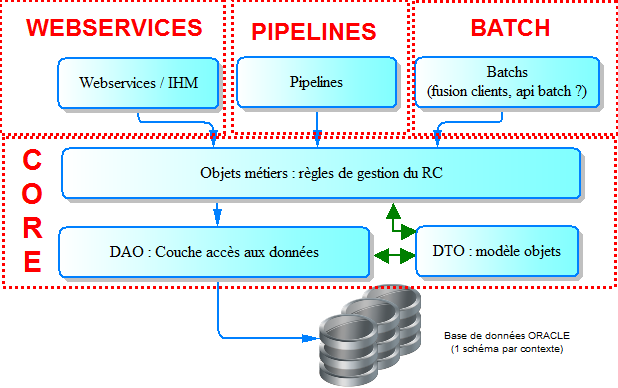
\includegraphics[width=\textwidth]{images/rc_arch_general.png}
\end{frame}

\begin{frame}{Modules du référentiel coordonnées}
	\begin{description}[<+->]
	\item[Core] Coeur de l'application (jar) :
		\begin{itemize}
		\item Modèle objets : représentation \emph{client} / \emph{coordonnées}
		\item couche d'accès au données : structure de la base, gestion des schémas
		\item règles de gestion : calcul des consentements, règles de mises à jour, dé-duplication
		\end{itemize}
	\item[Webservices] Application Java EE (war) exposant des webservices
		\begin{itemize}
		\item correspondance \emph{modèle objet interne} $\leftrightarrow$ \emph{contrat WSDL}
		\item Interface WEB : suivi des pipelines
		\end{itemize}
	\item[Pipelines] Intégration de données par fichiers CSV (jar exécutable)
		\begin{itemize}
		\item Démarrage/Arrêt d'un \emph{démon}
		\item Détection de l'arrivée de fichiers
		\item EAI et lecture de fichier
		\item Parallélisation des traitements
		\end{itemize}
	\item[Batch] Exports, traitements de types : fusion, statistiques, \dots
	\end{description}
\end{frame}


\subsection{Compilation et déploiement}

\begin{frame}{Organisation des modules}
	\framesubtitle{En utilisant \emph{Maven}}
	
	\begin{block}{Maven}
	\emph{Apache Maven} est un logiciel de gestion de projet. Basé sur le concept de \emph{Project Object Model} (POM), il gère le processus de compilation, rapports, \dots
	\end{block}
	
	\pause
	Le Référentiel Coordonnées utilise \emph{Maven} pour : 
	\begin{itemize}
	\item la gestion des dépendances
	\item le packaging : compilation, tests automatique, archives zip et ear
	\item le déploiement des pipelines et batch (FTP)
	\item configuration du poste de travail : \emph{Eclipse}
	\item tests en local des Webservices et IHM
	\end{itemize}

\end{frame}

\begin{frame}{Projets et sous-projets \emph{Maven}}
	
	Le référentiel coordonnées est répartie sur 6 projets \emph{Maven} :
	\begin{itemize}[<+->]
	\item \textbf{addressrepository} : \emph{version, dépendances, modules (pom)} 
		\begin{itemize}
		\item \textbf{address-core} : \emph{coeur de l'application} (jar)\par
		package : \texttt{net.yvesrocher.services.address.core}
		\item \textbf{address-pipelines} : \emph{démon (jar exécutable)}\par
		package : \texttt{net.yvesrocher.services.address.pipelines}
		\item \textbf{address-webservices} : \emph{War du webservices}\par
		package : \texttt{net.yvesrocher.services.address.webservices}
		\item \textbf{address-ear} : \emph{Package le war en un EAR}
		\item \textbf{address-batch} : \emph{Batchs utilisant le coeur V3 ( jar exécutable)}\par
		package : \texttt{net.yvesrocher.services.address.batch}
		\end{itemize}
	\end{itemize}

\end{frame}

\begin{frame}[fragile]{Compilation et déploiement}

	\begin{block}{Compilation}
	Maven exécute les tests unitaires et crée les binaires s'il n'y a pas d'erreur. Les binaires sont présents dans le répertoire \texttt{target} de chaque module.
	\end{block}
	
	\pause
	Commande Maven de compilation et déploiement sur FTP :
	\begin{lstlisting}
mvn clean install -DdeployPipelines
	\end{lstlisting}

\end{frame}


\section{Coeur applicatif}

\subsection{Configuration}

\begin{frame}{Configuration}
	\framesubtitle{Inversion de Contrôle, avec \emph{Spring} !}
	
	\begin{block}{Spring}
	Spring fournit l'inversion de contrôle : cycle de vie des \emph{beans}, injection de dépendances et gestion de la configuration.
	\end{block}
	
	\pause
	Les fichiers de configuration se trouvent dans \texttt{src/main/resources} :
	\begin{itemize}[<+->]
	\item \texttt{spring} : fichiers de configuration \emph{Spring} :
		\begin{itemize}[<+->]
		\item \texttt{addressrepository-core.xml} : inclue les fichiers nécessaires
		\item \texttt{addressrepository-businessservice.xml} : paramètre le coeur pour être intégré à un autre Webservice
		\end{itemize}
	\item \texttt{config} : fichiers de paramétrage (\emph{properties})
	\end{itemize}
	
\end{frame}

\subsection{Gestion des contextes}
% Scope "context"

\begin{frame}{Gestion des contextes du RC}
	\framesubtitle{Porté \emph{Spring} : \texttt{context}}
	
	\begin{block}{Scope \texttt{context}}
En plus des scopes classiques \texttt{singleton} et \texttt{prototype}, le scope \texttt{context} défini un singleton d'un contexte.	
	\end{block}
	
	\pause
	\begin{itemize}
	\item Seule une instance de bean contexté est créée pour chaque contexte.
	\end{itemize}


\end{frame}

\begin{frame}{Distribution sur les contextes}
	\framesubtitle{Une instance du coeur est créée pour chaque contexte}
	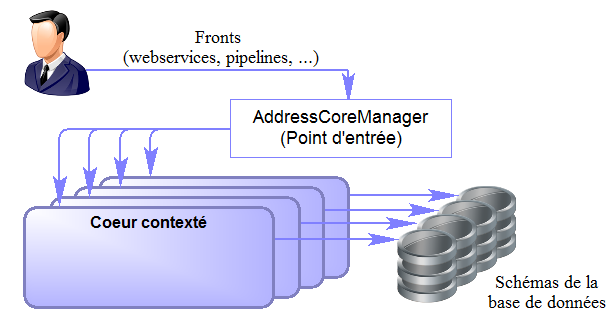
\includegraphics[width=\textwidth]{images/rc_arch_contexts.png}
\end{frame}


\subsection{Plan et principales briques logicielles}

\begin{frame}{Cartographie du coeur}
	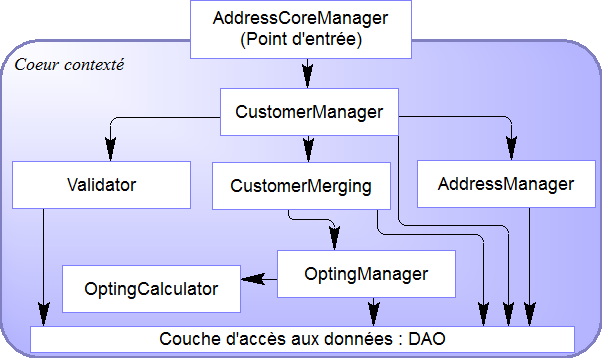
\includegraphics[width=\textwidth]{images/rc_arch_business.png}
%	[height=8cm]
\end{frame}

\begin{frame}{Briques applicatives du RC}

	\begin{itemize}
	\item \textbf{CustomerManager} Point d'entrée du coeur
		\begin{itemize}
		\item Exécute la validation
		\item Recherche les doublons
		\item Distribue : nouveau client, mise à jour, prospect
		\end{itemize}
	\item \textbf{Validator} Valide les données d'un client, de ses comptes et coordonnées.
	\item \textbf{AddressManager} Traitement des coordonnées prospectes.
	\item \textbf{CustomerMerging} Confronte les données présentes en base à la mise à jour
	\item \textbf{OptingManager} Règle générale sur les consentements (propagations, flag)
	\item \textbf{OptingCalculator} Calculs des consentements
	\end{itemize}
	
\end{frame}

\subsection{Couche d'accès au données}

\begin{frame}{Couche d'accès aux données}
	\framesubtitle{Object Relational Mapping par \emph{Hibernate}}
	
	\begin{block}{Hibernate}
	Le framework \emph{Hibernate} est utilisé pour gérer la relation entre le modèle objet et la base de données.
	\end{block}
	
	\pause
	\begin{block}{Session Factory}
	La \texttt{SessionFactory} d'Hibernate est configuré par Spring dans le fichier \texttt{context-persistence.xml}.\par
	Elle a pour scope le \textbf{context} : une session factory par schéma.	
	\end{block}

\end{frame}

\begin{frame}{Configuration des sources de données}

	Les sources de données sont fournie à \emph{Spring} par le \texttt{DatasourceProvider}. Il se repose sur 2 implémentations de \emph{IDatasourceFactory} :
	\begin{itemize}
	\item \texttt{FileDatasourceFactoryImpl} : fichier properties présent sur UNIX (pipelines, batch)
	\item \texttt{JndiDatasourceFactoryImpl} : datasources présentes dans un dictionnaire JNDI
	\end{itemize}

\end{frame}

\begin{frame}{Pattern : \emph{Open Session In View}}

	\begin{block}{Open Session In View}
	Le pattern \emph{Open Session In View} consiste à ouvrir la session le plus tôt possible, et la fermée le plus tard possible. Ainsi, les relations lazy ne sont chargées qu'au dernier moment et seulement si nécessaire.
	\end{block}
	
	\pause
	\begin{block}{Ouverture des sessions}
	L'annotation \texttt{$@$OpenSession} permet d'ouvrir la session pour la méthode annotée, ou toutes les méthodes de la classes annotée.
	\end{block}
	
	\pause
	\begin{block}{Transactions}
	En revanche, les transactions sont positionnées pour garantir la cohérence de la base de données. Elle sont configurée par l'annotation \texttt{$@$Transactional}
	\end{block}

\end{frame}

% Recherche des datasources
% Configuration de la session factory
% Pattern "open session in view"
% gestion des transactions

\subsection{API de tests unitaires}
% @DatabaseScripts

\begin{frame}{Tests unitaires dans le RC}
	\framesubtitle{Outils utilisés}
	
	\begin{description}[<+->]
	\item[JUNIT] Framework de tests unitaires
	\item[FestAssert] Écriture des assertions dans les tests
	\item[Mockito] Isole les beans business afin de pouvoir les isoler avant de les tester
	\item[HSQL] Base de données en mémoire vive pour tester les DAO
	\item[DBUnit] Charge/Décharge les données de tests dans la base HSQL
	\end{description}

\end{frame}

\begin{frame}{API de test}
	\framesubtitle{Éléments principaux de l'API}

	Éléments développés dans le RC pour faciliter l'écriture des tests
	\begin{itemize}[<+->]
	\item classes parentes pré-configurée
	\item sur-couche de \emph{DBUnit}
	\item assertions spécifique sur les DTO (avec \emph{FestAssert})
	\item méthodes de génération de données de tests
	\end{itemize}
\end{frame}

\begin{frame}{Classes parentes de tests unitaires}

	Classes principales à surcharger :
	\begin{itemize}[<+->]
	\item \textbf{SimpleJunitTest} : Super-classe principale des tests unitaire dans le RC. Initialise le contexte Spring
	\item \textbf{DBUnitTest} : Initialise la BDD HSQL et configure Hibernate pour l'utiliser
	\item \textbf{ContextedJunitTest} : permet l'injection de \emph{beans contextés} dans la classe de test
	\end{itemize}
\end{frame}

\begin{frame}{Sur-couche de DBUnit}
	\framesubtitle{Annotation \texttt{$@$DatabaseScripts}}
	
	\begin{block}{DBunit}
	DBunit est un outils chargeant, vidant ou exportant le contenu d'une BDD, à partir ou vers des fichiers XML.
	\end{block}
	
	\pause
	L'annotation \texttt{$@$DatabaseScripts}, développée pour le RC :
	\begin{itemize}
	\item positionnée sur les méthodes de tests, ou au niveau classe
	\item définit les fichiers à utiliser pour charger la BDD
	\item les \texttt{locations} sont héritées de la classe, et des classes parentes
	\item pas d'héritage si \texttt{inheritsLocations} est \texttt{true}
	\end{itemize}
\end{frame}

\section{Webservices et IHM}

\subsection{Module webservices RC}

\begin{frame}{Module webservices RC}

	\begin{block}{Module Webservices du RC}
	Ce module est déployé sur un serveur d'applications (type \emph{Websphère}).\par
	Il expose des webservices et fait le lien avec le coeur RC
	\end{block}
	
	\pause
	\begin{itemize}[<+->]
	\item Pas de logique métier en dehors de la règle A : seul le compte correspondant au réseau de l'appel est pris en compte.
	\item Package des classes non générées :\par
	\texttt{net.yvesrocher.services.address.webservices}
	\item la majorité du module sont les \emph{mapper} : DTO $\leftrightarrow$ WSDL
	\end{itemize}

\end{frame}


\subsection{IHM de monitoring}

\begin{frame}{IHM de monitoring}
	\framesubtitle{Avec \emph{Spring MVC}}
	
	\begin{block}{Spring MVC}
	\textbf{Dispatcher} : en fonction de l'URL d'appel, trouve la méthode la plus appropriée. La méthode réalise l'action et indique la vue à utiliser.	
	\end{block}
	
	\pause
	\begin{itemize}
	\item package des \emph{contrôleurs} :\par
	\texttt{net.yvesrocher.services.address.webservices.servlet. controller}
	\end{itemize}

\end{frame}


\section{Pipelines}

\subsection{Module Pipelines}

\begin{frame}{Module des pipelines}

	\begin{block}{Pipelines}
	Application \emph{standalone} de type démon. Elle détecte l'arrivée de fichiers, détermine leur type et les traite.
	\end{block}
	
	\pause
	Parties des pipelines :
	\begin{itemize}[<+->]
	\item \textbf{démon} : démarrage et arrêt de l'application
	\item \textbf{configuration} : quels sont les répertoires à scanner, quels traitements
	\item \textbf{gestion des traitements} : limite du nombre de traitements simultanés, global et par contexte
	\end{itemize}

\end{frame}

\subsection{Démon des pipelines}

\begin{frame}{Démon pipelines}

	\begin{block}{Démon}
	Déployé dans une archive ZIP, contient un jar, ses dépendances et son paramétrage : fichiers de configuration, fichiers \emph{scriptella}.\par
	La partie démon est implémenté dans la classe \texttt{main}.
	\end{block}

	\pause
	\begin{itemize}
	\item Écoute sur un port, configurable : \texttt{Socket TCP}
	\item Transmission de chaine de caractères à travers la \texttt{socket} pour arrêter le démon, connaitre sa version ou son état.
	\end{itemize}

	\pause
	\begin{exampleblock}{Évolutions possibles}
	Normaliser cette communication par RPC Java (Remote Procedure Call).
	\end{exampleblock}

\end{frame}

\subsection{Configuration}

\begin{frame}[containsverbatim]{Configuration des pipelines}
	\framesubtitle{Déclaration des flux d'entrée standard}
	
	\lstset{language=XML}
	\begin{lstlisting}
<pipelinesConfiguration>
	<dataInputs>
		<csvFileFlux id="classicCsv">
			<encoding>UTF-8</encoding>
			<separator>;</separator>
			<quote>''</quote>
		</csvFileFlux>
	</dataInputs>
	
	<pipelines>
		<!-- Pipelines standardises -->
		<pipeline enabled="true">
			<context>
				<brandId>YR</brandId>
				<countryId>RU</countryId>
			</context>
			<name>YR/RU/standard/update</name>
			<location>YRRU/standard</location>
			<discriminator>[A-Za-z]{4}_(SYN|REP|PRO)_.*</discriminator>
			<standardMethod />
		</pipeline>
		
	</pipelines>
</pipelinesConfiguration>
	\end{lstlisting}

\end{frame}


\begin{frame}[containsverbatim]{Configuration des pipelines}
	\framesubtitle{Déclaration d'un flux non standard}
	
	\lstset{language=XML}
	\begin{lstlisting}
...
		<pipeline enabled="true">
			<name>YR/RU/_reprise/isam</name>
			<location>YRRU/scriptella</location>
			<discriminator>[A-Za-z]{4}_REP_ISAM_.*</discriminator>
			<context>
				<brandId>YR</brandId>
				<countryId>RU</countryId>
				<language>ru</language>
			</context>
			<scriptellaMethod csvFile="classicCsv">
				<mapperScript>isam/reprise/isam_yrru.mapper.js</mapperScript>
				<nature>REPRISE</nature>
				<pipelineName>20_diamant</pipelineName>
				<properties>
					<processType>REPRISE</processType>
					<applicationCode>ISAM</applicationCode>
					<conCode>VPM</conCode>
					<pchCode>VPM</pchCode>
					<copScopeDefault>VPM</copScopeDefault>
					<bevCode>REP</bevCode>
					<styCode>SI</styCode>
					<copRequester>ISAM</copRequester>
				</properties>
			</scriptellaMethod>
		</pipeline>
...
	\end{lstlisting}

\end{frame}


\begin{frame}{Gestion des traitements}

	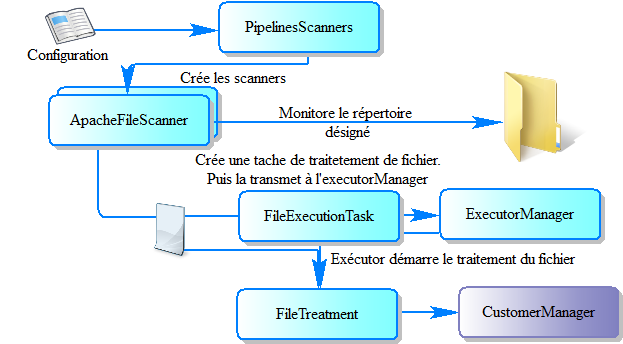
\includegraphics[width=\textwidth]{images/rc_pipelines.png}

\end{frame}

\lstset{language=JAVA}

% configuration
% timers
% plan des beans
% Exemple concret (diagrammes séquence)




\end{document}